%!TEX root = ../dokumentation.tex

\chapter{Ordnerstruktur}
\label{ch:Ordnerstruktur}
\begin{wrapfigure}{r}{.4\textwidth}
\centering
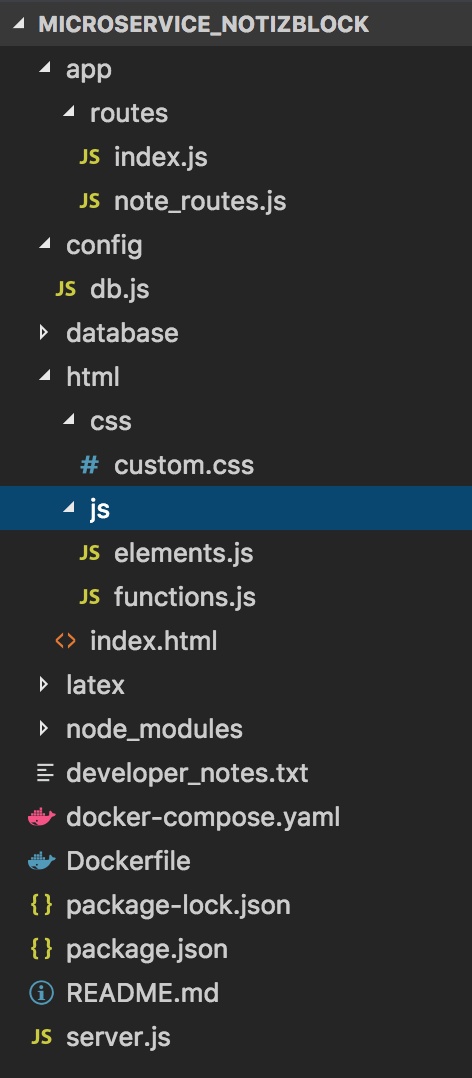
\includegraphics[height=.85\textwidth]{Ordnerstruktur.png}
\vspace{1pt}
\caption{Ordnerstruktur}
\label{fig:Ordnerstruktur}
\end{wrapfigure}

Der app-Ordner enthält die Routes der Anwendung. Diese beschreiben die einzelnen Pfade der \acs{CRUD}-Operationen.

Im config-Ordner befindet sich die \glqq db.js\grqq{}. Diese legt die Verbindung zur Mongo-Datenbank fest.

Der Ordner \glqq database\grqq{}wird für die Datenbank-Engine benötigt und enthält automatisch generierte Dateien, die mit der Installation des MongoDB-Treibers mit einher gehen.

Im \glqq \acs{HTML}\grqq{}-Ordner finden sich alle notwendigen Dateien für die Oberfläche der Anwendung. So ist das grundlegende html-File direkt in diesem Ordner abgelegt. Die zugehörigen Stylesheets befinden sich im \glqq \acs{CSS}\grqq{}-Ordner, die Javascript-Methoden im \acs{JS}-Ordner.

Im Ordner latex befinden sich die Dateien für die Dokumentation im latex-Format.

Der Ordner node\_modules wird durch das Kommando \glqq  npm install\grqq{} und die in der package.json festgelegten Dependencies automatisch befüllt.

Die Datei \glqq  developer\_notes.txt \grqq{} enthält Informationen über die Pfade zu den einzelnen Methoden der Anwendung.

Das \glqq docker-compose.yaml\grqq{} legt die Eigenschaften der Containerorchestrierung fest. Auf diesem File beruht das spätere Kommando \glqq  docker-compose up\grqq{} das die komplette Anwendung containerisiert startet.

Das Dockerfile legt das Image des Anwendungscontainer fest.
Die \glqq package.json\grqq{} beschreibt die Grundlagen der Anwendung und verzeichnet die Dependencies für den Node Package Manager.
Das \textit{README} wurde für den Upload auf Github erstellt und enthält eine kurze Beschreibung der relevanten Anwendungsschnittstellen.

Die \glqq server.js\grqq{}-Datei bildet das Herzstück der Anwendung. Hier werden die diversen Teile der Anwendung durch Imports bzw. Requirements zusammengeführt. Des Weiteren wird hier der Node-Server gestartet, sowie Anforderungen für verwendete Frameworks gesetzt.